\section{Experiment}
\subsection{Setup}

During the laboratory we used the SDG1025 signal generator and a "SDS1052DL+" oscilloscope.
\subsubsection*{Detailed explanation of how we used it}
SDG1025 signal generator
\begin{figure}[H]
	\centering
	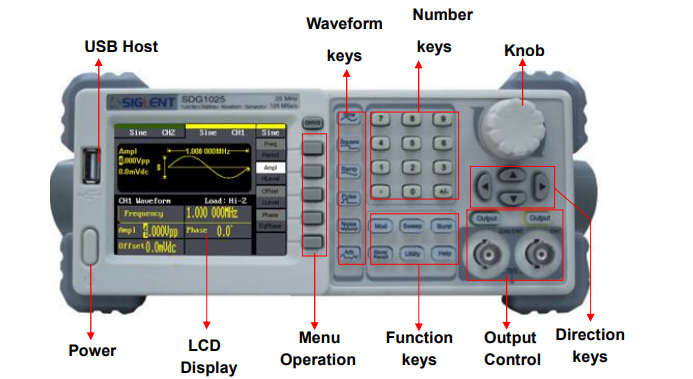
\includegraphics[width=10cm]{images/11.png}
	\caption{SDG1025}
	\label{fig:wow1}
\end{figure}

\begin{figure}[H]
	\centering
	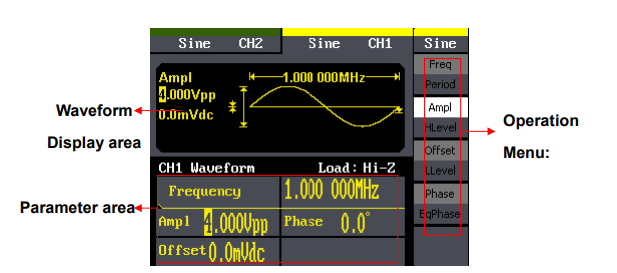
\includegraphics[width=10cm]{images/15.png}
	\caption{SDG1025 interface}
	\label{fig:wow5}
\end{figure}

\begin{itemize}
	\item To set a waveform we used buttons with a waveform icon that are on \textbf{"waveform keys"} panel.
	\item With "Sine" button waveform window will display sine waveform.
	\item By setting frequency/period, amplitude/high level, offset/low level, sine signal with different parameters can be generated.
	\item To set freq and another parameters we used \textbf{Number keys}, all parameters displayed in "\textbf{Parameter Area}"
	\item We used two buttons on the right side of the
   operation panel, which are used to activate or deactivate the output signal.
	\item There are three sets of buttons on the operation
  panel, which are direction button, the knob and the keypad.
	\item The up and down keys were used to shift parameters and the left and right
     keys were used to shift digits.
	\item Keypad was used to directly set the parameters value.
	\item Knob was used to change a signal digit value whose range is 0~9
\end{itemize}

\begin{figure}[H]
	\centering
	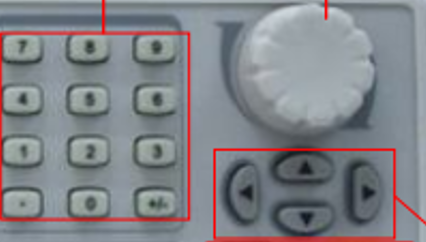
\includegraphics[width=10cm]{images/13.png}
	\label{fig:wow3}
\end{figure}

\begin{figure}[H]
	\centering
	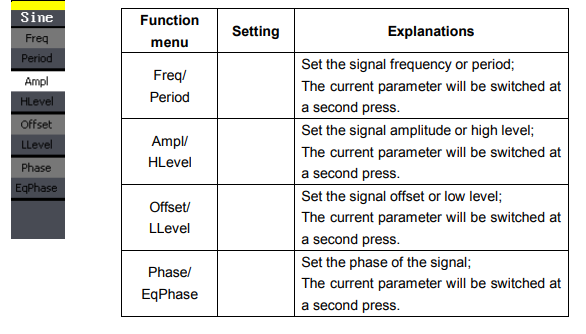
\includegraphics[width=10cm]{images/14.png}
	\caption{Setting sign signals}
	\label{fig:wow4}
\end{figure}

 - To Set the Output Frequency/Period we used "\textbf{Sine}" and "\textbf{Freq}" buttons.
   The frequency shown on the screen when the instrument is powered is
   the default value or the set value beforehand. When setting the function,
   if the current value is valid for the new waveform, it will be used
   sequentially. Also we used direction button to select the digit you want to edit and direction button to select the digit you want to edit.
 - We applied the same for the rest of the parameters using "\textbf{Ampl}", "\textbf{Offset}" and "\textbf{Phase}" buttons.

\subsubsection*{"SDS1052DL+" oscilloscope}
\begin{figure}[H]
	\centering
	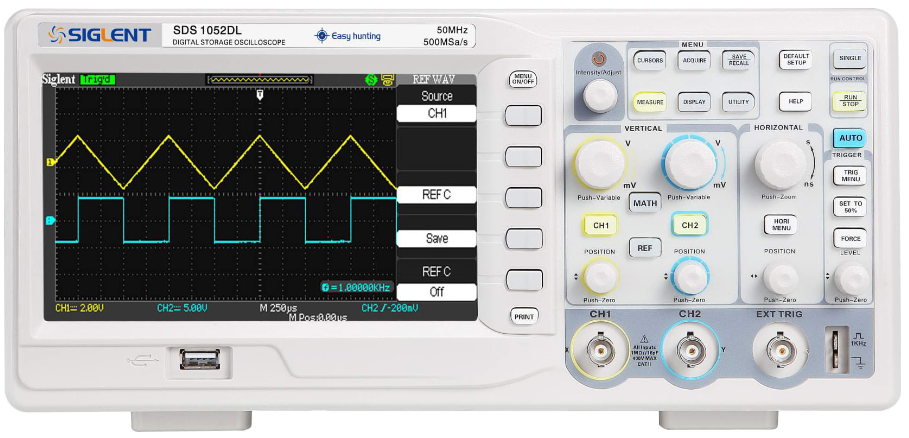
\includegraphics[width=10cm]{images/16.png}
	\caption{Schematic example}
	\label{fig:wow6}
\end{figure}

\subsubsection*{Menu and Control Button}
\begin{itemize}
	\item It would be better to start from channel buttons. We used them to turn that channel ON or OFF and open the channel menu for that channel. Also we can use the channel menu to
  set up a channel. When the channel is on, the channel button is lit.
	\item RUN/STOP: Continuously acquires waveforms or stops the acquisition.
	\item SET TO 50\unit{\percent}: We used it to stabilize a waveform quickly. The oscilloscope can set the trigger level to be halfway between the minimum and maximum
  voltage level automatically.
	\item MATH: It used to display the Math menu. We can use the "\textbf{MATH}" menu to use the
  oscilloscopes Math functions.
	\item "HORI MENU": We used it to display the Horizontal menu. We can use the Horizontal
  menu to display the waveform and zoom in a segment of a waveform.
	\item MEASURE: Used to display a menu of measurement parameters.
	\item AUTO: Very useful button. Automatically sets the oscilloscope controls to produce a usable display
  of the input signals.
	\item SINGLE: Acquire a single waveform and then stops.
	\item Channel Connector (CH1, CH2): Input connectors for waveforms display.
	\item The horizontal position control establishes the time between the trigger position
  and the screen center. We can adjust the horizontal “POSITION” knob control to
  view waveform data before the trigger, after the trigger, or some of each. When
  we change the horizontal position of a waveform, we are changing the time
  between the trigger and the center of the display actually
\end{itemize}

\subsubsection*{Universal Knob}

\begin{figure}[H]
	\centering
	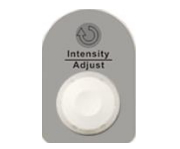
\includegraphics[width=10cm]{images/17.png}
	\caption{Universal knob}
	\label{fig:wow7}
\end{figure}

This is a very useful knob. We used the Universal knob with many functions, such as adjusting the
  holdoff time, moving cursors, setting the pulse width, adjusting the upper and lower frequency limit, adjust X and Y masks when
  using the pass/fail function etc. We can also turn the “Universal” knob to
  adjust the storage position of setups, waveforms, pictures when
  saving/recalling and to select menu options.

\subsubsection*{Vertical System}
We used vertical control for displaying waveform, rectify scale and
position.

\begin{figure}[H]
	\centering
	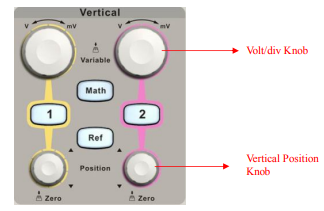
\includegraphics[width=10cm]{images/18.png}
	\label{fig:wow8}
\end{figure}


\subsubsection*{Horizontal System}
As shown on the picture below, there are one button and two knobs in the HORIZONTAL area.
We used the horizontal controls to change the horizontal scale and position of
waveforms. The horizontal position readout shows the time represented by the
center of the screen, using the time of the trigger as zero. Changing the horizontal
scale causes the waveform to expand or contract around the screen center.

\begin{figure}[H]
	\centering
	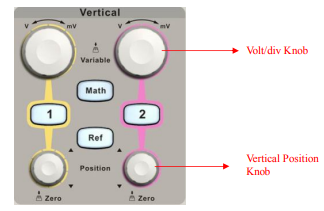
\includegraphics[width=10cm]{images/18.png}
	\label{fig:wow9}
\end{figure}

\subsection{Measurement methods}

First, we explored different ways of obtaining the parameters' values. We configured the signal generator to $f = \SI{864}{\hertz}$, $V_{pp} = \SI{2.6}{\volt}$ and connected it to the first oscilloscope channel.

\subsubsection*{Direct}

 To obtain parameters' values using the direct method, one must read the peak-to-peak distance from the oscilloscope's display and multiply it by the setting of the sensitivity knob. The picture may be shifted with knobs to facilitate reading.

The vertical sensitivity knob was set to \SI{0.5}{\volt}. Table~\ref{tab:direct-method} shows the parameters' values.

\begin{table}[H]
	\centering
	\begin{tabular}{c|c|c|c|c|c|c}
		$Y [div]$ & $C_{y} [\unit{\volt}]$ & $f [\unit{\hertz}]$ & $V_{pp} [\unit{\volt}]$ & $V_{m} [\unit{\volt}]$ & $V_{0} [\unit{\volt}]$ & $T [\unit{\micro\second}]$\\
		\hline
		5.1 & 0.5 & 864 & 2.55 & 1.275 & 0.3 & 1157
	\end{tabular}
	\caption{Direct method ($Y$ -- peak-to-peak distance, $C_{y}$ -- sensitivity, $f$ -- frequency, $V_{pp}$ -- peak-to-peak voltage, $V_{m}$ -- magnitude, $V_{0}$ -- average (DC) voltage, $T$ -- period)}
	\label{tab:direct-method}
\end{table}

$V_{pp}$, $V_{m}$ and $T$ calculations are shown in Equations~\ref{eq:peak-to-peak},~\ref{eq:magnitude},~\ref{eq:frequency}.


\begin{equation}
	V_{pp} = Y\cdot C_{y} = 5.1\cdot \SI{0.5}{\volt} = \SI{2.55}{\volt}
	\label{eq:peak-to-peak}
\end{equation}

\begin{equation}
	V_{m} = \frac{V_{pp}}{2} = \frac{\SI{2.55}{\volt}}{2} = \SI{1.275}{\volt}
	\label{eq:magnitude}
\end{equation}

\begin{equation}
	T = \frac{1}{f} = \frac{1}{\SI{864}{\hertz}} = \SI{0.001157407407}{\second} = \SI{1157}{\micro\second}
	\label{eq:frequency}
\end{equation}

\subsubsection*{Cursors}

In the cursors method, the measurement is performed indirectly via two pairs of horizontal and vertical cursors. The distance between a pair of cursors is displayed on the screen. Therefore, e.g. signal peak-to-peak voltage may be measured by aligning horizontal cursors with its opposite peaks.

The cursors were positioned at \SI{1.64}{\volt} and \SI{-0.96}{\volt}. Table~\ref{tab:cursors-method} shows the parameters' values.

\begin{table}[H]
	\centering
	\begin{tabular}{c|c|c|c|c|c|c}
		$V_{a} [\unit\volt]$ & $V_{b} [\unit\volt]$ & $f [\unit{\hertz}]$ & $V_{pp} [\unit{\volt}]$ & $V_{m} [\unit{\volt}]$ & $V_{0} [\unit{\volt}]$ & $T [\unit{\micro\second}]$\\
		\hline
		1.64 & -0.96 & 864 & 2.6 & 1.3 & 0.3 & 1157
	\end{tabular}
	\caption{Direct method ($V_{b}$ -- 1st cursor, $V_{b}$ -- 2nd cursor, $f$ -- frequency, $V_{pp}$ -- peak-to-peak voltage, $V_{m}$ -- magnitude, $V_{0}$ -- average (DC) voltage, $T$ -- period)}
	\label{tab:cursors-method}
\end{table}

$V_{m}$ and $T$ calculations are shown in Equations~\ref{eq:magnitude2},~\ref{eq:frequency2}.

\begin{equation}
	V_{m} = \frac{V_{pp}}{2} = \frac{\SI{2.6}{\volt}}{2} = \SI{1.3}{\volt}
	\label{eq:magnitude2}
\end{equation}

\begin{equation}
	T = \frac{1}{f} = \frac{1}{\SI{864}{\hertz}} = \SI{0.001157407407}{\second} = \SI{1157}{\micro\second}
	\label{eq:frequency2}
\end{equation}


\subsubsection*{Measure}

In the measure method, a "measure" button is pressed on the oscilloscope to obtain the results. The peak-to-peak value is then read directly from the display.

Table~\ref{tab:measure-method} shows the parameters' values.

\begin{table}[H]
	\centering
	\begin{tabular}{c|c|c|c|c}
		$f [\unit{\hertz}]$ & $V_{pp} [\unit{\volt}]$ & $V_{m} [\unit{\volt}]$ & $V_{0} [\unit{\volt}]$ & $T [\unit{\micro\second}]$\\
		\hline
		864 & 2.6 & 1.3 & 0.3 & 1157
	\end{tabular}
	\caption{Direct method ($f$ -- frequency, $V_{pp}$ -- peak-to-peak voltage, $V_{m}$ -- magnitude, $V_{0}$ -- average (DC) voltage, $T$ -- period)}
	\label{tab:measure-method}
\end{table}   

$V_{m}$ and $T$ calculations are shown in Equations~\ref{eq:magnitude3},~\ref{eq:frequency3}.

\begin{equation}
	V_{m} = \frac{V_{pp}}{2} = \frac{\SI{2.6}{\volt}}{2} = \SI{1.3}{\volt}
	\label{eq:magnitude3}
\end{equation}

\begin{equation}
	T = \frac{1}{f} = \frac{1}{\SI{864}{\hertz}} = \SI{0.001157407407}{\second} = \SI{1157}{\micro\second}
	\label{eq:frequency3}
\end{equation}

\subsection{Triggering}

In this part of the experiment we observed what happens to displayed signals when different trigger sources are used. We generated two signals and connected them to Channels 1 and 2.

\begin{itemize}
	\item CH1
	\begin{itemize}
		\item $V_{0} = \SI{0}{\volt}$
		\item $V_{pp} = \SI{2.3}{\volt}$
		\item $f = \SI{864}{\hertz}$ or $f = \SI{1}{\kilo\hertz}$
	\end{itemize}
	\item CH2
	\begin{itemize}
		\item $V_{0} = \SI{0}{\volt}$
		\item $V_{pp} = \SI{2}{\volt}$
		\item $f = \SI{4}{\kilo\hertz}$
	\end{itemize}
\end{itemize}

Next, different frequency and trigger combinations were tried. Table~\ref{tab:triggering} shows the collected data.

\begin{table}[H]
	\centering
	\begin{tabular}{c|c|c|c}
		$f_{1} [\unit{\kilo\hertz}]$ & $f_{2} [\unit{\kilo\hertz}]$ & Trigger source & Graph\\
		\hline
		0.864 & 4 & CH1 & Unstable\\
		\hline
		1 & 4 & CH1 & Stable\\
		\hline
		1 & 4 & CH2 & Unstable\\
		\hline
		0.864 & 4 & CH2 & Unstable\\
	\end{tabular}
	\caption{Frequency and trigger combinations}
	\label{tab:triggering}
\end{table}

\subsection{Oscilloscope functions}
In the last part of the experiment we investigated two functions offered by the device: Math and Acquire.

The Math function facilitates performing operations such as signal addition, subtraction, multiplication, etc.

The Acquire function is used to control how the waveform is generated by varying the sample rate of the ADC (analog-to-digital) converter, and offers various acquisition modes. During the laboratory we used the Averaging Acquisition Mode - it averaged out the noise in the taken samples and displayed the underlying signal.
